To implement the desired algorithm we need to be able to calculate the optical behavior of stacked Meta Surfaces. The mathematical framework we will use is called Scatter Matrix Calculus and this section will give some insight into its physical origin and how to use it. We will start at the very beginning with the Maxwell Equations in matter.
\newlparagraph{Maxwell Equations}


\noindent
\begin{tabular*}{\textwidth}{ll}
\begin{minipeqn}
    \curl{\vb{E}(\vb{r}, t)} = - \pdv{t} \vb{B}(\vb{r}, t)
\end{minipeqn}&
\begin{minipeqn}[c]
    \div \vb{D}(\vb{r}, t) = \rho_\s{ext}(\vb r, t)
\end{minipeqn}\\
\begin{minipeqn}
    \curl \vb H(\vb r, t) = \vb j(\vb r, t) + \pdv{t} \vb D(\vb r, t)
\end{minipeqn}&
\begin{minipeqn}[c]
    \div \vb B(\vb r, t) = 0
\end{minipeqn}
\end{tabular*}
\\
\\


\noindent
The four involved fields are:
$\vb E$...electric field, $\vb B$...magnetic flux density, $\vb D$...electric flux density and $\vb H$...magnetic field and the sources are the external charges $\rho_\s{ext}$ and the macroscopic currents $j$. All the material properties are captured by the $\vb D$ and $\vb H$ fields which are defined as follows:
\\

\begin{equation}\label{eq:bg:D}
\begin{aligned}
    \vb D(\vb r, t) &= \varepsilon_0 \vb E (\vb r, t) + \vb P (\vb r, t)\\
    \vb H(\vb r, t) &= \frac{1}{\mu_0} \qty[\vb B(\vb r, t) - \vb M(\vb r, t)]
\end{aligned}
\end{equation}


Where $\vb P$ is the dielectric polarization and $\vb M$ is the magnetic polarisation. One can read equation \ref{eq:bg:D} in the following way:
When the electric field $\vb E$ interacts with matter it exerts a force on all its charges and displaces them by a small amount. The separation of charges results in a counter field $\vb P$ and the total field $\vb D$ is now a superposition of $\vb E$ and $\vb P$.
This set of equations describes the whole electromagnetic spectrum, in this work however we are only interested in visible (VIS) and near infra red (NIR) light so we can make some simplifications. $\rho_\s{ext}$ = 0 and $\vb M = 0$ \note{why?}. Inserting these assumptions into the maxwell equation gives:


\noindent
\begin{tabular*}{\textwidth}{ll}
\begin{minipeqn}\label{eq:bg:M1}
    \curl{\vb{E}(\vb{r}, t)} = - \mu_0 \pdv t \vb H(\vb r, t)
\end{minipeqn}&
\begin{minipeqn}[c]\label{eq:bg:M2}
    \varepsilon_0 \div \vb{E}(\vb{r}, t) = - \div \vb P(\vb r, t)
\end{minipeqn}\\
\begin{minipeqn}\label{eq:bg:M3}
    \curl \vb H(\vb r, t) = \vb j(\vb r, t) + \pdv{t} \vb P(\vb r, t)
    + \varepsilon_0 \pdv{t} \vb E(\vb r, t)
\end{minipeqn}&
\begin{minipeqn}[c]
    \div \vb H(\vb r, t) = 0
\end{minipeqn}
\end{tabular*}


\newlparagraph{Light in Vacuum}
Now we can derive the famous wave equation by considering $\curl$ \eqref{eq:bg:M1}:


\begin{equation}
\begin{aligned}
    \hspace{2.5cm}
    \curl \bigg [\curl \vb E \bigg ] &= \curl[- \mu_0 \pdv t \vb H]\\
    \hspace{2.5cm}
    \Leftrightarrow
    \grad(\div \vb E) - \Delta \vb E &=
    - \mu_0 \pdv t \curl \vb H
    \qquad \bigg | \qq{subs. \eqref{eq:bg:M3} and \eqref{eq:bg:M2}}
    \\
    \hspace{2.5cm}
    \Leftrightarrow
    \frac{1}{c^2} \pdv[2] t \vb E - \Delta \vb E
    &= -\mu_0 \pdv t \vb j - \mu_0 \pdv[2] t \vb P +
    \frac{1}{\varepsilon_0} \grad(\div \vb P)
\end{aligned}
\end{equation}

In vacuum ($\vb P = 0$ and $\vb j = 0$) the right side of this equation vanishes and we are left with\\
$\frac{1}{c^2} \pdv[2] t \vb E - \Delta \vb E = 0$ which is solved by the plane wave $\vb E = \vb E_0 e^{i(\vb k \vb r - \omega t)}$ where $\frac{\omega}{k} = c$. This describes the propagation of light through empty space: a sinusoidal occilation in time and space along the $\vb k$ direction where $\vb E, \, \vb B$ and $\vb k$ are all perpendicular to each other.
\note{this needs details} \note{show figure?}

\newlparagraph{Light in homogeneous, isotropic materials}
\noindent
The next question we can answer is how light propagates through a homogeneous and isotropic material. For us the dielectric polarization is some linear function of the electric field so $\vb P(\vb r, t) = \hat{\chi}(\omega, \vb r) \vb E(\vb r, t)$. An isotropic material behaves the same for all orientations of $\vb E$ that means $\hat{\chi}(\omega, \vb r)$ becomes a scalar property $\chi(\omega, \vb r)$. If the material is additionally homogeneous, that is the same everywhere independent of $\vb r$, then $\div \chi(\omega, \vb r) = 0$. With equation \eqref{eq:bg:M2} this gives us $\div \vb P = 0$
and the wave equation simplifies to \note{why is j=0}:

\begin{equation}
\begin{aligned}
    &\frac{\varepsilon}{c^2} \pdv[2] t \vb E - \Delta \vb E = 0\\
    \qq*{where} &\varepsilon \, \vb E := \qty(1 + \chi) \vb E = \vb E + \vb P
\end{aligned}
\end{equation}

So light behaves in these materials exactly as it would in vacuum we only have to account for a decreased speed of light
$c' = \frac{c}{\sqrt{\varepsilon}} =: \frac{c}{n}$
with the refractive index $n$.
This is equivalent to a decreased wavelength
$\lambda' =: \frac{\lambda}{n}$
which results in an increased wave vector
$k' = \frac{2 \pi}{\lambda'} = n \, k$
A complex valued $n := \eta + i \kappa$ even captures the possibility of a decaying field:

\begin{equation}
    \vb E = \vb E_0 e^{i(n \vb k \vb r - \omega t)}
    = \vb E_0 \
    \underbrace{e^{-\kappa \vb k \vb r}}_\s{
    decay} \
    \underbrace{e^{i(\eta \vb k \vb r - \omega t)}}_\s{
    oscillation}
\end{equation}

\newlparagraph{Interfaces}
The meta surface stacks we want to understand are obviously not one homogeneous material. Rather they contain many interfaces between different materials and we can again use the maxwell equations to predict how light will behave at such an interface.
\\

\begin{figure}[H]
    \centering
    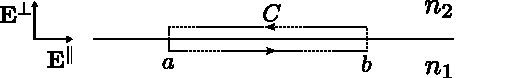
\includegraphics[width=.6\linewidth]{bg_interface}
    \caption{An interface of two materials with different refractive indices $n_1$ and $n_2$}
    \label{fig:bg:interface}
\end{figure}

Let us consider a closed contour $C$ around an interface as seen in Figure \ref{fig:bg:interface} and integrate the first maxwell equation \eqref{eq:bg:M1} over the surface $A$ enclosed by that contour:

\begin{equation}
\begin{aligned}
    \int_A \curl \vb E(\vb r, t) \, \dd \vb A
    &= - \mu_0 \pdv t \int_A \vb H(\vb r, t) \dd \vb A\\
    \overset{\s{stokes}}{\Longleftrightarrow} \hspace{3em}
    \int_{C = \partial A} \vb E(\vb r, t) \dd \vb r
    &= - \mu_0 \pdv t \int_A \vb H(\vb r, t) \dd \vb A\\
\end{aligned}
\end{equation}

Now we can bring the contour infinitely close to the interface and thus reduce the right hand side of the equation, the total magnetic flux\note{?} through the surface, to zero. That leaves us with:

\begin{equation}
\begin{aligned}
    \int_a^b \vb E_1 \, \dd \vb r \ &+ \int_b^a \vb E_2 \,  \dd \vb r = 0\\
    \Longleftrightarrow \hspace{3em}
    \int_a^b \vb E_1 \, \dd \vb r &= \int_a^b \vb E_2 \,  \dd \vb r \\
\end{aligned}
\end{equation}

Because $a$ and $b$ were also chosen arbitrarily that means that the transverse field components along the path need to be continuous so
$\vb E_1^{\parallel} = \vb E_2^{\parallel}$.
The analog expression
$\vb H_1^{\parallel} = \vb H_2^{\parallel}$
can be shown by starting with the first maxwell equation \eqref{eq:bg:M1} instead.

\begin{figure}[H]
    \centering
    \includegraphics[width=.7\linewidth]{bg_fresnel}
    \caption{Interface between two materials of different refractive indices $n_1$ and $n_2$. Shown is an incident wave with wave vector $\vb k_\s{i}$ which is partially transmitted and partially reflected.}
    \label{fig:bg:fresnel}
\end{figure}

Let us consider the same interface from before and have an incident field
$\vb E^\s{i}$ interact with it. From figure \ref{fig:bg:fresnel} we can see:

\begin{equation} \label{eq:bg:k}
    \vb k^\s{i} = k_0 n_1
    \begin{pmatrix}
        -\sin \varphi_\s{i}\\ 0\\ -\cos \varphi_\s{i}
    \end{pmatrix}
    , \
    \vb k^\s{r} = k_0 n_1
    \begin{pmatrix}
        \phantom{-} \sin \varphi_\s{r} \\ 0\\ -\cos \varphi_\s{r}
    \end{pmatrix}
    , \
    \vb k^\s{r} = k_0 n_2
    \begin{pmatrix}
        \sin \varphi_\s{t}\\ 0\\ \cos \varphi_\s{t}
    \end{pmatrix}
\end{equation}

Now we can decompose the electric field into a component were $\vb E = E \, \va{e_y}$ called transverse electric (TE) and its orthogonal component where $\vb H = H \, \va{e_y}$ called transverse magnetic (TM). If we apply the continuity condition from before on the TE component we get $\vb E_1 = \vb E_2$ at $z = 0$:

\begin{equation}
\begin{aligned}
    \vb E^\s{i} + \vb E^\s{r} &= \vb E^\s{t} \\
    E^\s{i} e^{i(k^\s{i}_x x)} + E^\s{r} e^{i(k^\s{r}_x x)}
    &= E^\s{t} e^{i(k^\s{t}_x x)}
\end{aligned}
\end{equation}

This is only possible for all $x$ if:

\begin{equation}
    E^\s{i} + E^\s{r} = E^\s{t} \qq{and}
    k^\s{i}_x = k^\s{r}_x = k^\s{t}_x
\end{equation}

Two basic laws of optics lie in this relation: The law of reflection \note{fix the signs}

\begin{equation}
    k^\s{i}_x = k^\s{r}_x
    \quad \Rightarrow \quad
    - k_0 n_1 \sin \varphi_i =  k_0 n_1 \sin \varphi_r
    \quad \Rightarrow \quad
    \varphi_i = \varphi_r
\end{equation}

and the Snells law of refraction

\begin{equation}
    k^\s{i}_x = k^\s{t}_x
    \quad \Rightarrow \quad
    - k_0 n_1 \sin \varphi_i =  k_0 n_2 \sin \varphi_t
    \quad \Rightarrow \quad
    n_1 \sin \varphi_i = n_2 \sin \varphi_t
\end{equation}

\newlparagraph{Fresnel Equations}
To fully describe an interface we also need know the fraction of the transmitted
$t := \frac{\vb E^t}{\vb E^i}$
and the reflected
$r := \frac{\vb E^r}{\vb E^i}$ fields.
We are still only considering the TE polarization for the derivation. Here as $\vb E = E \, \va e_y$ the $\vb H$ field has both $x$ and $z$ components and only $\vb H_x$ has to follow the continuity condition because it is oriented  transverse to the interface:

\begin{equation}
    \vb H^\s{i}_x + \vb H^\s{r}_x = \vb H^\s{t}_x \\
\end{equation}

Using the third maxwell equation \eqref{eq:bg:M3} this $\vb H_x$ component can be expressed by the electric field:

\begin{equation}
\begin{aligned}
    \quad \phantom{\Rightarrow} \quad
    \curl \vb E_0 e^{i(\vb k \vb r - \omega t)} &=
    \varepsilon_0 \pdv t \vb H_0 e^{i(\vb k \vb r - \omega t)} \\
    \quad \Rightarrow \quad
    \vb k \times \vb E_0 e^{i(\vb k \vb r - \omega t)} &=
    \varepsilon_0 \omega \ \vb H_0 e^{i(\vb k \vb r - \omega t)} \\
    \quad \Rightarrow \quad
    \vb k \times \vb E_0 &=
    \varepsilon_0 \omega \ \vb H_0 \\
    \quad \Rightarrow \quad
    \vb H_{0x} =
    \frac{1}{\varepsilon_0 \omega} \ \qty(\vb k \times \vb E_0)_x
    &\stackrel{\eqref{eq:bg:k}}{=}
    \frac{1}{\varepsilon_0 \omega} \\

\end{aligned}
\end{equation}
